Töö tulemusena valmis avalikult kättesaadav veebirakendus \footnote{\url{https://tallinn.simplytobo.eu}}. Veebilehel valmis töö lõpuks mitu alamlehte. Töö lähtekood on avalikult kättesaadav. \footnote{\url{https://github.com/Tsarter/TallinnTransport}}

\section{Avalik andmebaas}

Kõik töö käigus kogutud andmed on avalikult kättesaadavad \footnote{\url{https://tallinn.simplytobo.eu/transport_data/}}. See võimaldab igal asjast huvitatud inimesel uurida Tallinna ühistransporti ja kuidas see on ajas muutunud. Antud töö raames ehitas autor mitmeid vahelehti just selle andmebaasi peale. Valminud lehtedest tuleb detailsemalt juttu järgmistes peatükkides. 

\section{Kiirused kaardil}\label{section:Kiirused-kaardil}

Pilte, kus kuvatud kiiruseid linnakaardil, on loodud näiteks Bostoni \cite{boston_woodruff_mbta_2011} ja Helsingi trammivõrgu jaoks \cite{jlf_tram_speeds}. Siin töös loodi sarnane interaktiivne kaart.

\begin{figure}[h!]
    \centering
    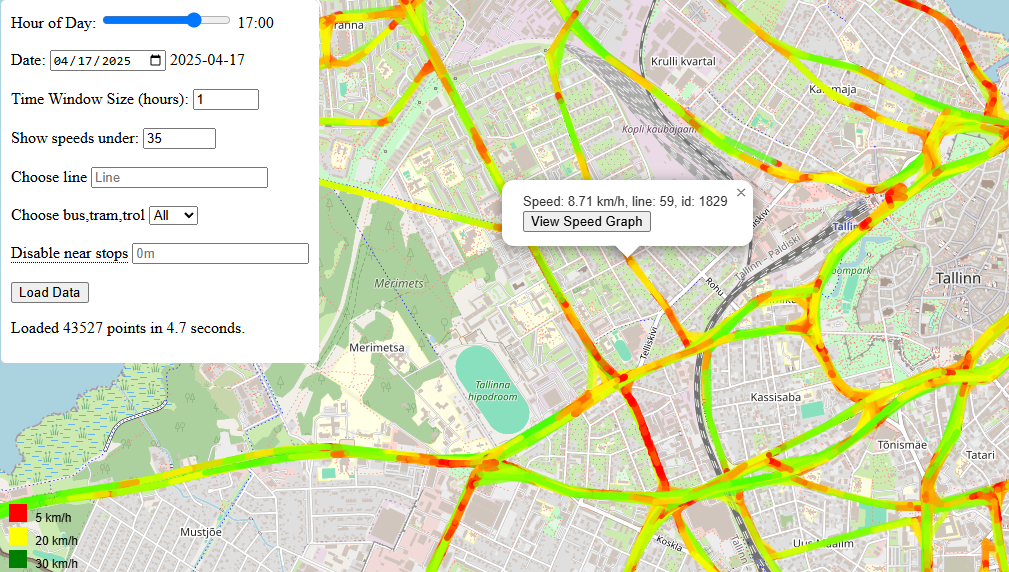
\includegraphics[width=0.8\textwidth]{figures/speedSegmentMap2.png}
    \caption{Kiirusi kuvav kaart. }
    \label{fig:Kiirustekaart}
\end{figure}

Joonisel \ref{fig:Kiirustekaart} on näha tallinna ühistranspordi sõidukite kiirusi neljandal aprillil aastal 2025 kella 17:00 - 18:00 vahel. Veebilehe kasutajal on võimalik valida kuupäev ja kellaaeg ning mitme tunni andmeid soovitakse näha. Aitamaks paremini näha aeglaseid kohti on võimalik välja filtreerida segmente kiiruse järgi. Soovides vaadelda konkreetset liini on seda võimalik teha sisestades vastava liini sümboli vastavasse kasti. Valides ka sõidukitüübi, saab tulemuse veelgi täpsemaks ja kuigi 1.november 2024 kadusid liinidelt trollid on antud rakenduses nende valimise võimalus olemas, kuna andmeid hakati koguma varem \cite{trollid}. Viimase võimalusena on võimalik välja jätta kõik segmendid, mis on ühistranspordi peatuste lähedal. Kasutaja saab sisestada numbri meetrites, mille järel ei näidata segmente, mis on lähemal. See aitab paremini näha fooride ja ristmike juures olevaid aeglaseid kohti. Andmete laadimiseks tuleb vajutada nuppu, mille järel saab näha kui palju andmeid laeti ja kui kiiresti.

Kollasega on segmendid, mille kiirus on 20 km/h lähedal. Seda kuna Lisa 2 andmetel on see ühissõidukite keskmine kiirus. Punasega on sellest allpool olevad kiirused ja rohelisega sellest ülevalpool olevad kiirused.

Igale kaardil olevale segmendile saab vajutada, et näha lisainformatsiooni. Selleks on kiirus, liin ja sõiduki identifikaator ning veelgi täpsemalt saab informatsiooni teada, kui vajutada nupule, kus on kirjas \textit{View Speed Graph}.

\section{Kiirused graafikul} 

Nägemaks paremini, kuidas kiirused päeva lõikes ühel liinil muutuvad, loodi vastav vaade. See avaneb, kui vajutada Joonisel \ref{fig:Kiirustekaart} mõne värvilise sektsiooni peale.

\begin{figure}[h]
    \centering
    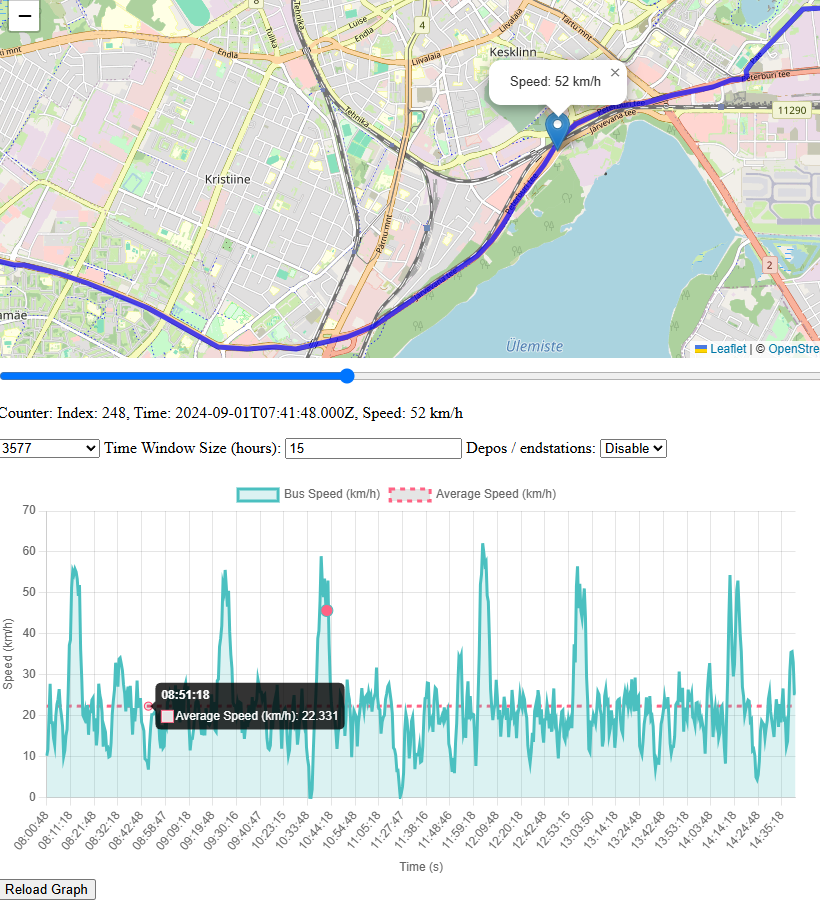
\includegraphics[width=0.8\textwidth]{figures/speedgraphDepos.png}
    \caption{Ühe sõiduki ühe päeva kiiruste graafik ja vastav kaart.}
    \label{fig:KiirusedGraafik}
\end{figure}

Joonisel \ref{fig:KiirusedGraafik} on näha bussiliini number 12 sõidukit identifikaatoriga 3577 1.septembril aastal 2024. Leheküljel on näha kaarti koos sõiduki marsruudiga, infot kellaaja ja hetkekiiruse kohta ning graafikut kiirustega. Graafikul on punase joonena kuvatud keskmist kiirust. 
Lehel on omavahel ühenduses kaart ja graafik. Lohistades sinist nuppu vasakule või paremale liigub punane täpp graafikul vastavasse kohta. Samal ajal liigub kaardil olev nupp kohta, kus sõiduk tol hetkel oli. Sedasi on näite puhul näha, et kui kiirused on suured, siis sõiduk asub Järvevana teel. Graafiku ajajoont jälgides on näha, et ajavahemikud ei ole ühtlased. Seda seetõttu, kuna lõpppeatustes ja depoos seismised on välja lõigatud. Juhul kui kasutaja soovib neid siiski näha on see võimalik seades \textit{Disable} nupu väärtuseks \textit{Enable}.


\section{Kahe punkti vaheline statistika} 

Saamaks paremat arusaama, kui kaua võtab aega ühistranspordil ühest kohast teise jõudmine, loodi vastav võimalus.

\begin{figure}[h!]
    \centering
    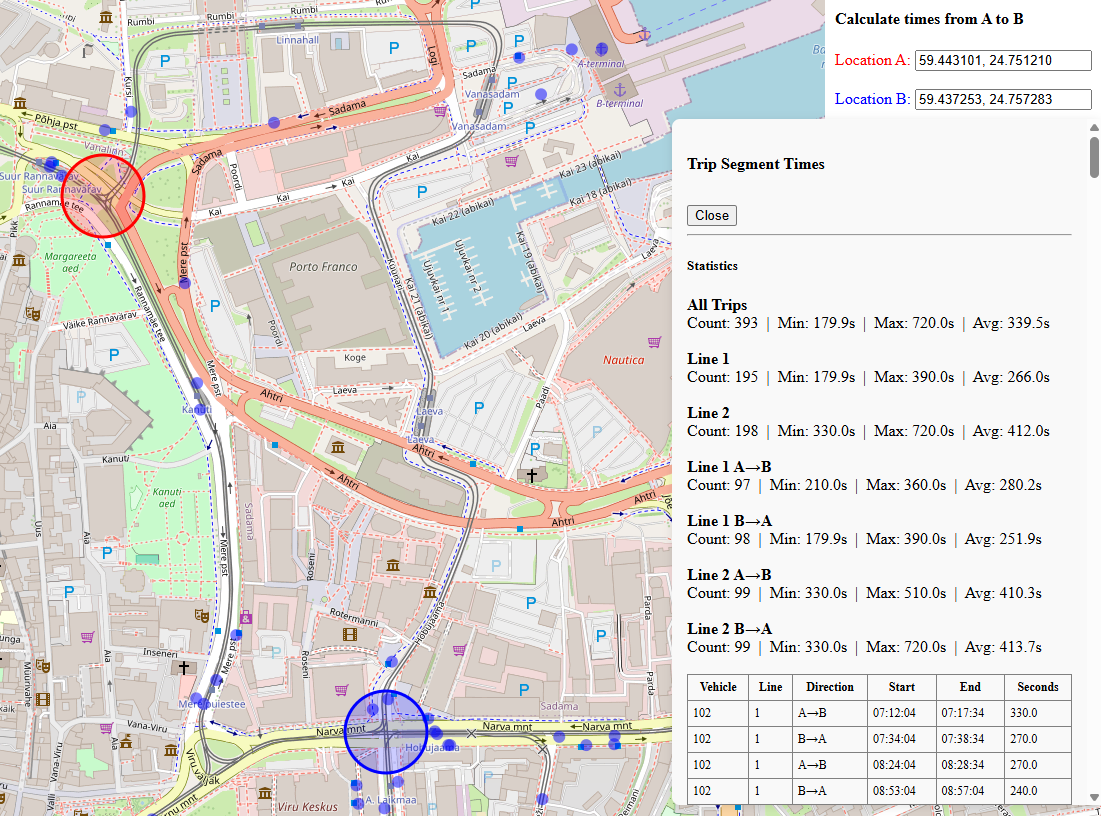
\includegraphics[width=0.8\textwidth]{figures/Liin1VsLiin2V2.png}
    \caption{Punkti A ja punkti B vahel liikunud sõidukite statistika.}
    \label{fig:Liin1VsLiin2V2}
\end{figure}

Võimalik on kaardile panna kaks ringi. Punane ring märgib punkti A ja sinine punkti B. Mõlema ringi raadius on 50 m. Andmebaasi päringu abil leitakse sõidukite teekonnad, mis läbisid neid kahte ringi. Statistika sektsioonis arvutatakse seejärel iga liini tuvastatud sõitude arv ning maksimaalne, minimaalne ja keskmine ajakulu. Lisaks näidatakse ka suuna põhiselt ehk punktist A punkti B kulunud aeg ja vastupidi. Kõige all on toodud ka kõik tuvastatud liikumised kahe punkti vahel tabelina välja. Selle tabeli saab kopeerida muude tarkvarasse, et sobivaid töötlusi veelgi teha. Näiteks saab vaadelda, kuidas ajakulu päeva lõikes muutub.


\section{Tallinna ühistranspordi keskmine kiirus}

Joonisel \ref{fig:KiirusedGraafik} on näha punast keskmise kiiruse joont. Selle info saab kätte iga liini kohta. Seda teadmist kasutades arvutati välja 2025. aasta märtsi sõidukite keskmised kiirused, mis on toodud välja Lisas 2.

Päringu tegemine võttis aega 20 minutit ja on seega aeglasema poolne. Autor on katsetanud eraldi tabeli tegemist taoliste päringute jaoks, mille tulemusel tehti sama päring alla sekundi. Kahjuks pole see lõplikult valmis ja on plaanis valmis teha tulevikus. Seetõttu pole keskmiste kiiruste infot ka avalikul veebilehel.

Katsetati ka muude päringute tegemist. Joonisel \ref{fig:nadalaKeskmine} on näha, kuidas tööpäeva alguses ja lõpus on kiirused madalamad kui tööpäeva keskel. Viimased kaks päeva on laupäev ja pühapäev ja seal on näha, et keskmine kiirus on päeva võrdluses ühtlasem. 
\begin{figure}[H]
    \centering
    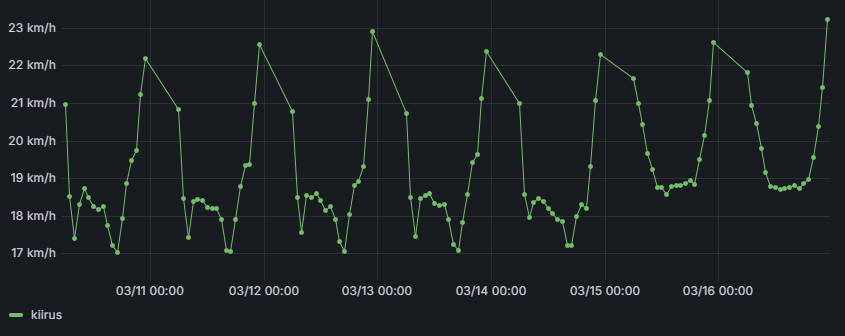
\includegraphics[width=0.9\textwidth]{figures/Kiirused5toopaeva2puhke.png}
    \caption{Kõikide ühissõidukite keskmiste kiiruste graafik ühe nädala vaates.}
    \label{fig:nadalaKeskmine}
\end{figure}





\section{Valideerimine}\label{section:valideerimine}

Tulemuste valideerimiseks võeti 4 bussi ja 1 trammi andmed. Kasutades Joonisel \ref{fig:KiirusedGraafik} näidatud tööriista pandi kirja, millal sõiduk algpeatusest väljus ja millal lõpppeatusesse jõudis. Google Earth'i \footnote{Liini pikkus~\url{https://earth.google.com/earth/d/1MccSsVoqKMNkUlBNQT4JodIoemFo2Ic8?usp=sharing}} abil leiti marsruudi ligikaudne pikkus.

Järgnevalt on näitena toodud ühe liini\footnote{Graafik leitav~\url{https://tallinn.simplytobo.eu/speedgraph/speedgraph.html?line=4&type=tram&vehicle_id=535&startTime=2025-04-14}} valideerimise protsess. 

\begin{longtable}{|l|c|c|c|c|c|c|}
\caption{14. aprillil trammiliinil 4 sõitnud trammi 535 sõidud.}
\label{tab:valideeringLiin4}\\ \hline % Sets a label for the table and starts the table with a horizontal line
\textbf{Väljumine}  &  \textbf{Saabumine} & \textbf{Aeg} & \textbf{Vahemaa} & \textbf{Kiirus} & \textbf{Alguspunkt} & \textbf{Sihtpunkt} \\ \hline
\endfirsthead
\hline
\textbf{Väljumine}  &  \textbf{Saabumine} & \textbf{Aeg} & \textbf{Vahemaa} & \textbf{Kiirus} & \textbf{Alguspunkt} & \textbf{Sihtpunkt} \\ \hline
\endhead
5:40:09 & 5:46:09  & 6 min & 2,1 km & 21,0 km/h & Pärnu mnt. depoo & Tondi \\ \hline
5:50:09 & 6:19:09  & 29 min & 7,6 km & 15,5 km/h & Tondi & Suur-Paala \\ \hline
6:31:39 & 6:59:39 & 28 min & 7,4 km & 16,1 km/h & Suur-Paala & Tondi \\ \hline
7:08:09 & 7:41:39  & 33,5 min & 7,6 km & 13,4 km/h & Tondi & Suur-Paala \\ \hline
7:48:09 & 8:19:09  & 32 min & 7,4 km & 14,1 km/h & Suur-Paala & Tondi \\ \hline
8:27:39 & 8:59:39  & 32 min & 7,6 km & 14,1 km/h & Tondi & Suur-Paala \\ \hline
9:19:39 & 9:49:09 & 29,5 min & 7,4 km & 15,2 km/h & Suur-Paala & Tondi \\ \hline
9:58:39 & 10:33:39  & 35 min & 7,6 km & 12,9 km/h & Tondi & Suur-Paala \\ \hline
10:49:39 & 11:19:09 & 29,5 min & 7,4 km & 15,2 km/h & Suur-Paala & Tondi \\ \hline
11:27:39 & 12:01:09  & 33,5 min & 7,6 km & 13,4 km/h & Tondi & Suur-Paala \\ \hline
12:10:39 & 12:40:39  & 30 min & 7,4 km & 15,0 km/h & Suur-Paala & Tondi \\ \hline
12:49:09 & 13:22:09  & 33 min & 7,6 km & 13,6 km/h & Tondi & Suur-Paala \\ \hline
13:31:09 & 14:01:09  & 30 min & 7,4\,km & 15,0 km/h & Suur-Paala & Tondi \\ \hline
14:05:39 & 14:12:09  & 6,5 min & 2,1 km & 19,4 km/h & Tondi & Pärnu mnt. depoo \\ \hline
\end{longtable}
Aeg tähendab siin aega, mis veedeti liinil olles. Iga marsruudi lõppu ja algusesse on seatud 75m suurune puhverala, mille sees olevaid mõõtmisi ei arvestata. See tähendab ka, et tabelis \ref{tab:valideeringLiin4} näitab vahemaa distantsi, mis läbiti ühest puhveralast teise jõudmiseks.

Käsitsi arvutamise järgi kulus 94,2 km läbimiseks 6 tundi ja 27 minutit. Keskmiseks kiiruseks saadi sel juhul 94,2 km / 6,45 h = 14.6 km/h. Automaatse skripti järgi sõideti 90,7 km ning liinil oldi 6 tundi ja 25 minutit ja keskmiseks kiiruseks saadi 14,2 km/h. 

Tegu on umbes 4 protsendilise erinevusega. Tegu ei ole suure eksimusega, kuid siiski on erinevus olemas. Nii automaatse skriptiga kui käsitsi saadud tulemused erinesid 2 minuti võrra ehk inimvea piires. 
Vahemaa erines 3,5 kilomeetriga. Seda mõningast viga võib põhjustada asjaolu, et asukohaandmed pole päris täpsed ehk kurvid võetakse sirgemaks. Joonisel \ref{fig:KiirusedGraafik} oleva tööriista järgi vaadeldi kurve. Näiteks Joonisel \ref{fig:kurvsirgeks} on viga kuskil 50 m. Arvestades, et tramm sõitis edasi-tagasi 12 korda, siis halvimal juhul tekkis ühes kurvis viga umbes 500 m. Trammiliinil 4 on kolm järsemat kurvi peatuste Lubja, Majaka ja Hobujaama lähedal, lisaks mitmeid laugemaid. Ehk 90 km peale võis sealt tekkida arvestatav viga. Selle lahendamiseks saaks asukohad tõsta teadaoleva marsruudi peale \cite{buenosAires}. Kahjuks jääb see töö mahust välja ja autor lepib teatud veaga kurvide arvutamisel.  

Järgnevalt valideeriti veel nelja erineva bussiliini andmeid. Lisas 2 on välja arvutatud 2025. aasta märtsi liinide liikumiskiirused. Selle abil valiti kõige kiirem bussiliin ehk 38, kõige aeglasem ehk 2 ja lisaks valiti ekspressliin 9, mille marsruut paistis ilma suuremate kurvideta. Bussiliin 81 valiti, kuna oli eelnevalt trolliliin.

\begin{longtable}{|l|c|c|c|c|c|c|}
\caption{Tulemuste valideerimine valitud sõidukite põhjal. Number 1 märgistab automaatse skripti tulemusi ja number 2 käsitsi valideerimisel saadud tulemusi. }
\label{tab:valideerimine}\\ \hline % Sets a label for the table and starts the table with a horizontal line
\textbf{Päev} & \textbf{Liin / id} & \textbf{Vahemaa 1} & \textbf{Vahemaa 2} & \textbf{Kiirus 1} & \textbf{Kiirus 2 } & \textbf{Viga} \\ \hline
\endfirsthead
\hline
\textbf{Päev} & \textbf{Liin / id} & \textbf{Vahemaa 1} & \textbf{Vahemaa 2} & \textbf{Kiirus 1} & \textbf{Kiirus 2 } & \textbf{Viga} \\ \hline
\endhead
2025-04-14 & 4 tramm / 535  & 90,7 km & 94,2 km & 14,2 km/h & 14,6 km /h & -3,7\% \\ \hline
2025-04-10 & 81 buss / 2669  & 214,9 km & 224,0 km & 16.0 km/h & 16.7 km/h & -4,2\% \\ \hline

2025-04-14 & 38 buss / 3320  & 126,1 km & 131,2 km & 25,9 km/h & 27.1 km /h & -4,4\% \\ \hline
2025-03-04 & 2 buss / 3535  & 155,8 km & 154,8 km & 15,6 km/h & 15,7 km /h & -0,6\% \\ \hline
2025-04-14 & 9 buss / 1813  & 160,1 km & 162,8 km & 22,8 km/h & 23,3 km /h & -2,1\% \\ \hline
\end{longtable}

Aegade võrdlusel ei leitud märkimisväärseid erinevusi ja seetõttu pole neid andmeid Tabelis \ref{tab:valideerimine}. Ainult bussiliini 2 mõõtmiste puhul oli märkimisväärne vahe, kus automaatne skript ei eemaldanud depoosse sõitu ja arvestas seda keskmise kiiruse arvutamisel. Kui see eemaldada tuleks vahemaa 149,8 km ja keskmine kiirus 15,2 km/h ning viga -3,2\%.
Liinide puhul esineb arvestav arv olukordi, kus depoost või depoosse sõitu ei lõigata välja. See muudab keskmist kiirust suuremaks. Kuna kurvide sirgeks lõikamine jälle vähendab keskmist kiirust, siis pikema perioodi jooksul need ilmselt mõnevõrra tühistavad üksteist. Samas ei saa sellele loota, kuna osade liinide lõpppeatused asuvad kohe depoo kõrval (nt bussiliin 9) ja seal ei tõsta depoosse sõit keskmist kiirust.

Bussiliini 38 puhul tuli viga kõige suurem, mis on tõenäoliselt seotud kurvilise ja kiire marsruudiga Pirita ja Viimsi teedel. Bussiliini 9 puhul tuli viga kõige väiksem ja see on ilmselt kuna Lasnamäelt Mustamäele sõidul pole järske kurve. 

Kuid üldpildis on kõik tulemused väga lähedal Lisas 2 leitud kiirustele. Kiiremad sõidukid ongi kiiremad ja aeglasemad aeglasemad. Seega peab autor leitud kiirusi õigeks, kuid paar protsenti liiga aeglaseks.
